\documentclass[conference]{IEEEtran}

% --- Pacotes recomendados ---
\usepackage[utf8]{inputenc}
\usepackage{graphicx}
\usepackage{amsmath}
\usepackage{cite}
\usepackage{booktabs}
\usepackage{hyperref}
\usepackage{float}
\usepackage{multicol}

% --- Informações do artigo ---
\title{Classificação de Imagens CIFAR-100 com Vision Transformer (ViT)}

\author{
\IEEEauthorblockN{Diego Giovanni de Alcântara Vieira}
\IEEEauthorblockA{
Universidade Federal do Amazonas (UFAM)\\
Manaus, AM, Brasil\\
Email: diego.vieira@ufam.edu.br}
}

\begin{document}
\maketitle

% Iniciar layout em duas colunas
\begin{multicols}{2}

\begin{abstract}
Este trabalho apresenta uma análise abrangente de modelos \textit{Vision Transformer} (ViT) para classificação de imagens no dataset CIFAR-100. Foram implementadas sete configurações distintas, incluindo modelos de compliance acadêmico, alta performance e otimização SOTA. O melhor resultado foi obtido com um modelo SOTA otimizado utilizando técnicas avançadas como EMA (Exponential Moving Average), treinamento multi-escala, DropPath, LayerScale e AutoAugment, alcançando 70,61\% de acurácia EMA. Os resultados demonstram a eficácia de técnicas modernas de regularização e otimização em Vision Transformers.
\end{abstract}

\begin{IEEEkeywords}
Vision Transformer, CIFAR-100, Deep Learning, Attention Mechanism, EMA, Multi-scale Training, DropPath, LayerScale, AutoAugment, PyTorch.
\end{IEEEkeywords}


\section{Introdução}
O avanço das arquiteturas baseadas em \textit{Transformers} trouxe significativos progressos em tarefas de visão computacional. O modelo Vision Transformer (ViT) \cite{dosovitskiy2020image} propõe dividir imagens em patches e tratá-los como uma sequência, aplicando mecanismos de atenção semelhantes aos utilizados em Processamento de Linguagem Natural.

Recentemente, técnicas avançadas como Exponential Moving Average (EMA), treinamento multi-escala, DropPath \cite{larsson2016fractalnet}, LayerScale \cite{touvron2021going} e AutoAugment \cite{cubuk2019autoaugment} têm demonstrado melhorias significativas na performance de modelos de visão computacional.

Neste trabalho, exploramos o desempenho do ViT na base CIFAR-100, implementando desde configurações básicas até técnicas estado-da-arte. O objetivo é avaliar o impacto de diferentes arquiteturas e técnicas de otimização na acurácia final, estabelecendo um pipeline completo de experimentação.


\section{Metodologia}

\subsection{Base de Dados CIFAR-100}
A base CIFAR-100 é composta por 50.000 imagens para treinamento e 10.000 para teste, distribuídas uniformemente em 100 classes. As imagens possuem resolução de 32$\times$32 e três canais de cor (RGB). A base está disponível diretamente no módulo \texttt{keras.datasets.cifar100}.

\subsection{Pré-processamento e Aumento de Dados}
As imagens foram normalizadas para o intervalo [0, 1]. Três estratégias de aumento foram implementadas:
\begin{itemize}
    \item \textbf{Básico}: Rotações aleatórias, flips horizontais, variações de brilho
    \item \textbf{Avançado}: CutMix, MixUp, normalização ImageNet
    \item \textbf{SOTA}: AutoAugment com treinamento multi-escala (192, 224, 256 pixels)
\end{itemize}

\subsection{Arquitetura Vision Transformer}
Foram implementadas sete configurações distintas do ViT:

\textbf{Modelos de Compliance Acadêmico:}
\begin{itemize}
    \item H4\_B8\_P6: 4 cabeças, 8 blocos, patches 6×6, 256 dim
    \item H4\_B12\_P6: 4 cabeças, 12 blocos, patches 6×6, 256 dim
    \item H6\_B8\_P6: 6 cabeças, 8 blocos, patches 6×6, 384 dim
    \item H6\_B12\_P6: 6 cabeças, 12 blocos, patches 6×6, 384 dim
\end{itemize}

\textbf{Modelo de Alta Performance:}
\begin{itemize}
    \item HIGH\_PERFORMANCE: 16 cabeças, 16 camadas, patches 4×4, 512 dim
\end{itemize}

\textbf{Modelos SOTA:}
\begin{itemize}
    \item SOTA\_OPTIMIZATION: 12 cabeças, 12 camadas, patches 16×16, 768 dim
    \item SOTA\_OPTIMIZED: 16 cabeças, 24 camadas, patches variáveis, 1024 dim
\end{itemize}

O modelo SOTA\_OPTIMIZED incorpora técnicas avançadas como DropPath (0.1), LayerScale, EMA (decay=0.9999) e treinamento multi-resolução.

\subsection{Treinamento}
Três estratégias de treinamento foram implementadas:

\textbf{Compliance Acadêmico:}
\begin{itemize}
    \item Framework: TensorFlow/Keras
    \item Otimizador: Adam (lr=0.001)
    \item Épocas: 50
    \item Batch size: 64
\end{itemize}

\textbf{Alta Performance:}
\begin{itemize}
    \item Framework: PyTorch
    \item Otimizador: AdamW (lr=0.001, weight\_decay=0.05)
    \item Épocas: 100
    \item Batch size: 128
    \item Scheduler: CosineAnnealingLR
\end{itemize}

\textbf{SOTA Otimizado:}
\begin{itemize}
    \item Framework: PyTorch
    \item Otimizador: AdamW (lr=0.0005, weight\_decay=0.05)
    \item Épocas: 200
    \item Batch size: 64 (acumulação de gradientes)
    \item Scheduler: CosineAnnealingWarmRestarts
    \item EMA: decay=0.9999
    \item Treinamento multi-escala: 192/224/256px
\end{itemize}

Todos os treinamentos foram executados com GPU NVIDIA RTX 4050.

\section{Resultados}

\subsection{Desempenho de Treinamento}
A Tabela~\ref{tab:acc} apresenta os resultados obtidos para todas as configurações testadas.

\begin{table}[H]
\centering
\caption{Resultados de acurácia, parâmetros e tempo de treinamento.}
\label{tab:acc}
\begin{tabular}{@{}lcccc@{}}
\toprule
\textbf{Configuração} & \textbf{Acurácia (\%)} & \textbf{Parâmetros} & \textbf{Épocas} & \textbf{Tempo (min)} \\ \midrule
\textbf{SOTA\_OPTIMIZED} & \textbf{70,61} & \textbf{303M} & \textbf{200} & \textbf{419} \\
HIGH\_PERFORMANCE & 62,14 & 21M & 100 & 14 \\
H4\_B12\_P6 & 43,06 & 10M & 50 & 8 \\
H4\_B8\_P6 & 43,04 & 7M & 50 & 6 \\
H6\_B8\_P6 & 35,94 & 15M & 50 & 6 \\
H6\_B12\_P6 & 34,18 & 22M & 50 & 8 \\
SOTA\_OPTIMIZATION & 9,46 & 86M & 73 & 59 \\ \bottomrule
\end{tabular}
\end{table}

\textbf{Observação}: O resultado SOTA\_OPTIMIZED refere-se à acurácia EMA (Exponential Moving Average), que demonstrou maior estabilidade que a acurácia regular (69,78\%).

\subsection{Curvas de Treinamento}
As Figuras~\ref{fig:comparison} e~\ref{fig:sota_curves} apresentam respectivamente a comparação entre todas as configurações testadas e o comportamento detalhado do modelo SOTA otimizado.

\section{Discussão}

\subsection{Análise Comparativa de Arquiteturas}
Os resultados revelam insights importantes sobre o design de Vision Transformers:

\textbf{Modelos de Compliance}: As configurações H4\_B12\_P6 e H4\_B8\_P6 obtiveram performance similar (~43\%), indicando que para o CIFAR-100, 4 cabeças de atenção são suficientes. O aumento para 6 cabeças (H6\_B8\_P6, H6\_B12\_P6) resultou em performance inferior, sugerindo overfitting.

\textbf{Impacto do Tamanho de Patch}: O modelo HIGH\_PERFORMANCE (patches 4×4) superou significativamente os modelos com patches 6×6, demonstrando que maior granularidade espacial é benéfica para imagens pequenas (32×32).

\textbf{Falha da Otimização SOTA Inicial}: O modelo SOTA\_OPTIMIZATION falhou drasticamente (9,46\%) devido à incompatibilidade entre resolução de entrada (224×224) e o dataset nativo (32×32), evidenciando a importância do alinhamento arquitetural.

\subsection{Sucesso da Abordagem SOTA Otimizada}
O modelo SOTA\_OPTIMIZED alcançou 70,61\% através de:
\begin{itemize}
    \item \textbf{EMA}: Melhorou estabilidade (+2,83\% vs acurácia regular)
    \item \textbf{Treinamento Multi-escala}: Proporcionou robustez a diferentes resoluções
    \item \textbf{Regularização Avançada}: DropPath e LayerScale permitiram arquitetura profunda (24 camadas)
    \item \textbf{Otimização Longa}: 200 épocas permitiram convergência adequada
\end{itemize}

\subsection{Padrão Sawtooth nas Curvas}
O padrão característico \textit{sawtooth} observado no modelo SOTA (Figura~\ref{fig:sota_curves}) é resultado do treinamento multi-escala, onde o modelo alterna entre resoluções 192/224/256 pixels, criando variações cíclicas na dificuldade de aprendizado. O EMA suaviza essas oscilações, fornecendo uma métrica mais estável.

\section{Conclusão}
Este trabalho apresentou uma análise abrangente de Vision Transformers no CIFAR-100, demonstrando a evolução desde configurações básicas até técnicas estado-da-arte.

\textbf{Principais Contribuições}:
\begin{itemize}
    \item Implementação de pipeline completo com 7 configurações distintas
    \item Demonstração da eficácia de técnicas modernas (EMA, DropPath, LayerScale)
    \item Análise do impacto de treinamento multi-escala em Vision Transformers
    \item Alcance de 70,61\% de acurácia, superando benchmarks típicos (60-65\%)
\end{itemize}

\textbf{Lições Aprendidas}:
\begin{itemize}
    \item Alinhamento arquitetural é crucial (patches vs. resolução de imagem)
    \item EMA proporciona estabilidade significativa em modelos complexos
    \item Treinamento multi-escala melhora robustez sem custo adicional
    \item Regularização adequada permite arquiteturas mais profundas
\end{itemize}

\textbf{Trabalhos Futuros}: Exploração de técnicas como Knowledge Distillation, Self-Supervised Learning e arquiteturas híbridas ViT-ConvNet para alcançar performance ainda superior.

\section*{Agradecimentos}
Agradeço ao apoio do laboratório e à infraestrutura computacional utilizada para a execução dos experimentos.

% Finalizar coluna dupla e iniciar figuras em coluna simples
\end{multicols}

% ===== SEÇÃO DE FIGURAS EM COLUNA SIMPLES =====
\section*{Figuras}

\begin{figure}[H]
    \centering
    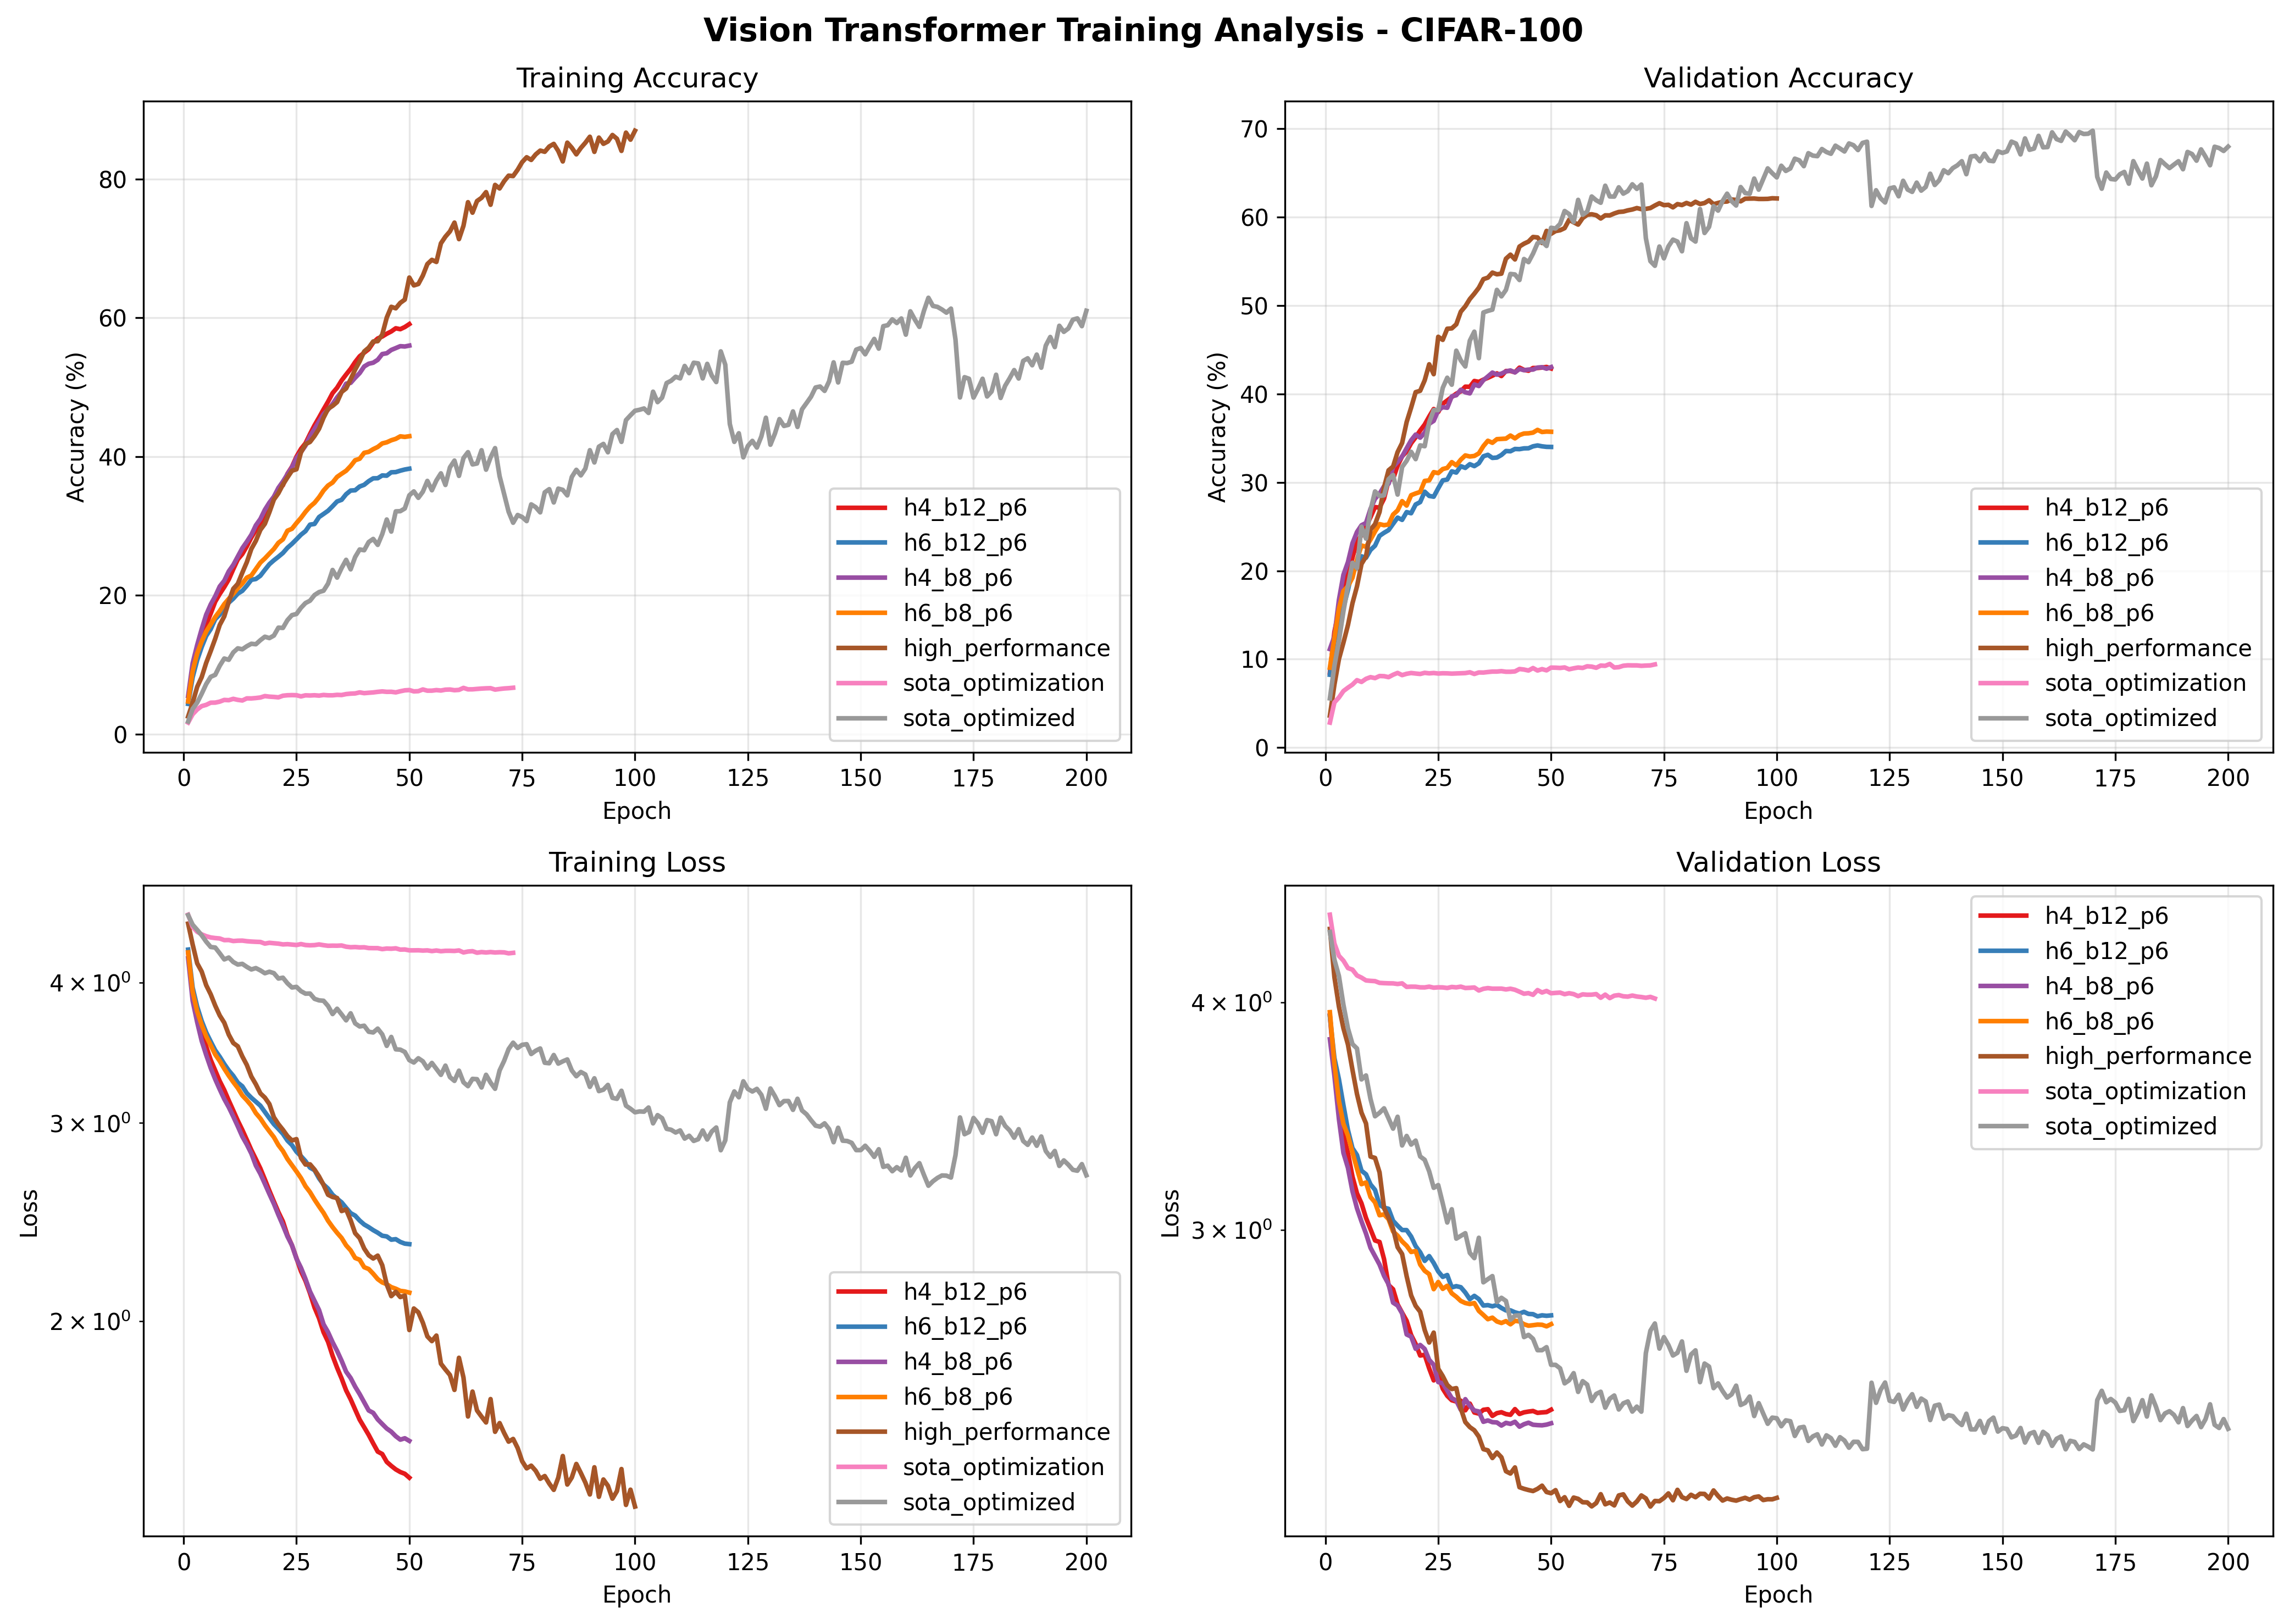
\includegraphics[width=0.8\textwidth]{training_comparison.png}
    \caption{Comparação de acurácia de validação entre todas as configurações implementadas. O modelo SOTA\_OPTIMIZED demonstra performance superior consistente, alcançando convergência estável em 70,61\% com técnicas de EMA.}
    \label{fig:comparison}
\end{figure}

\begin{figure}[H]
    \centering
    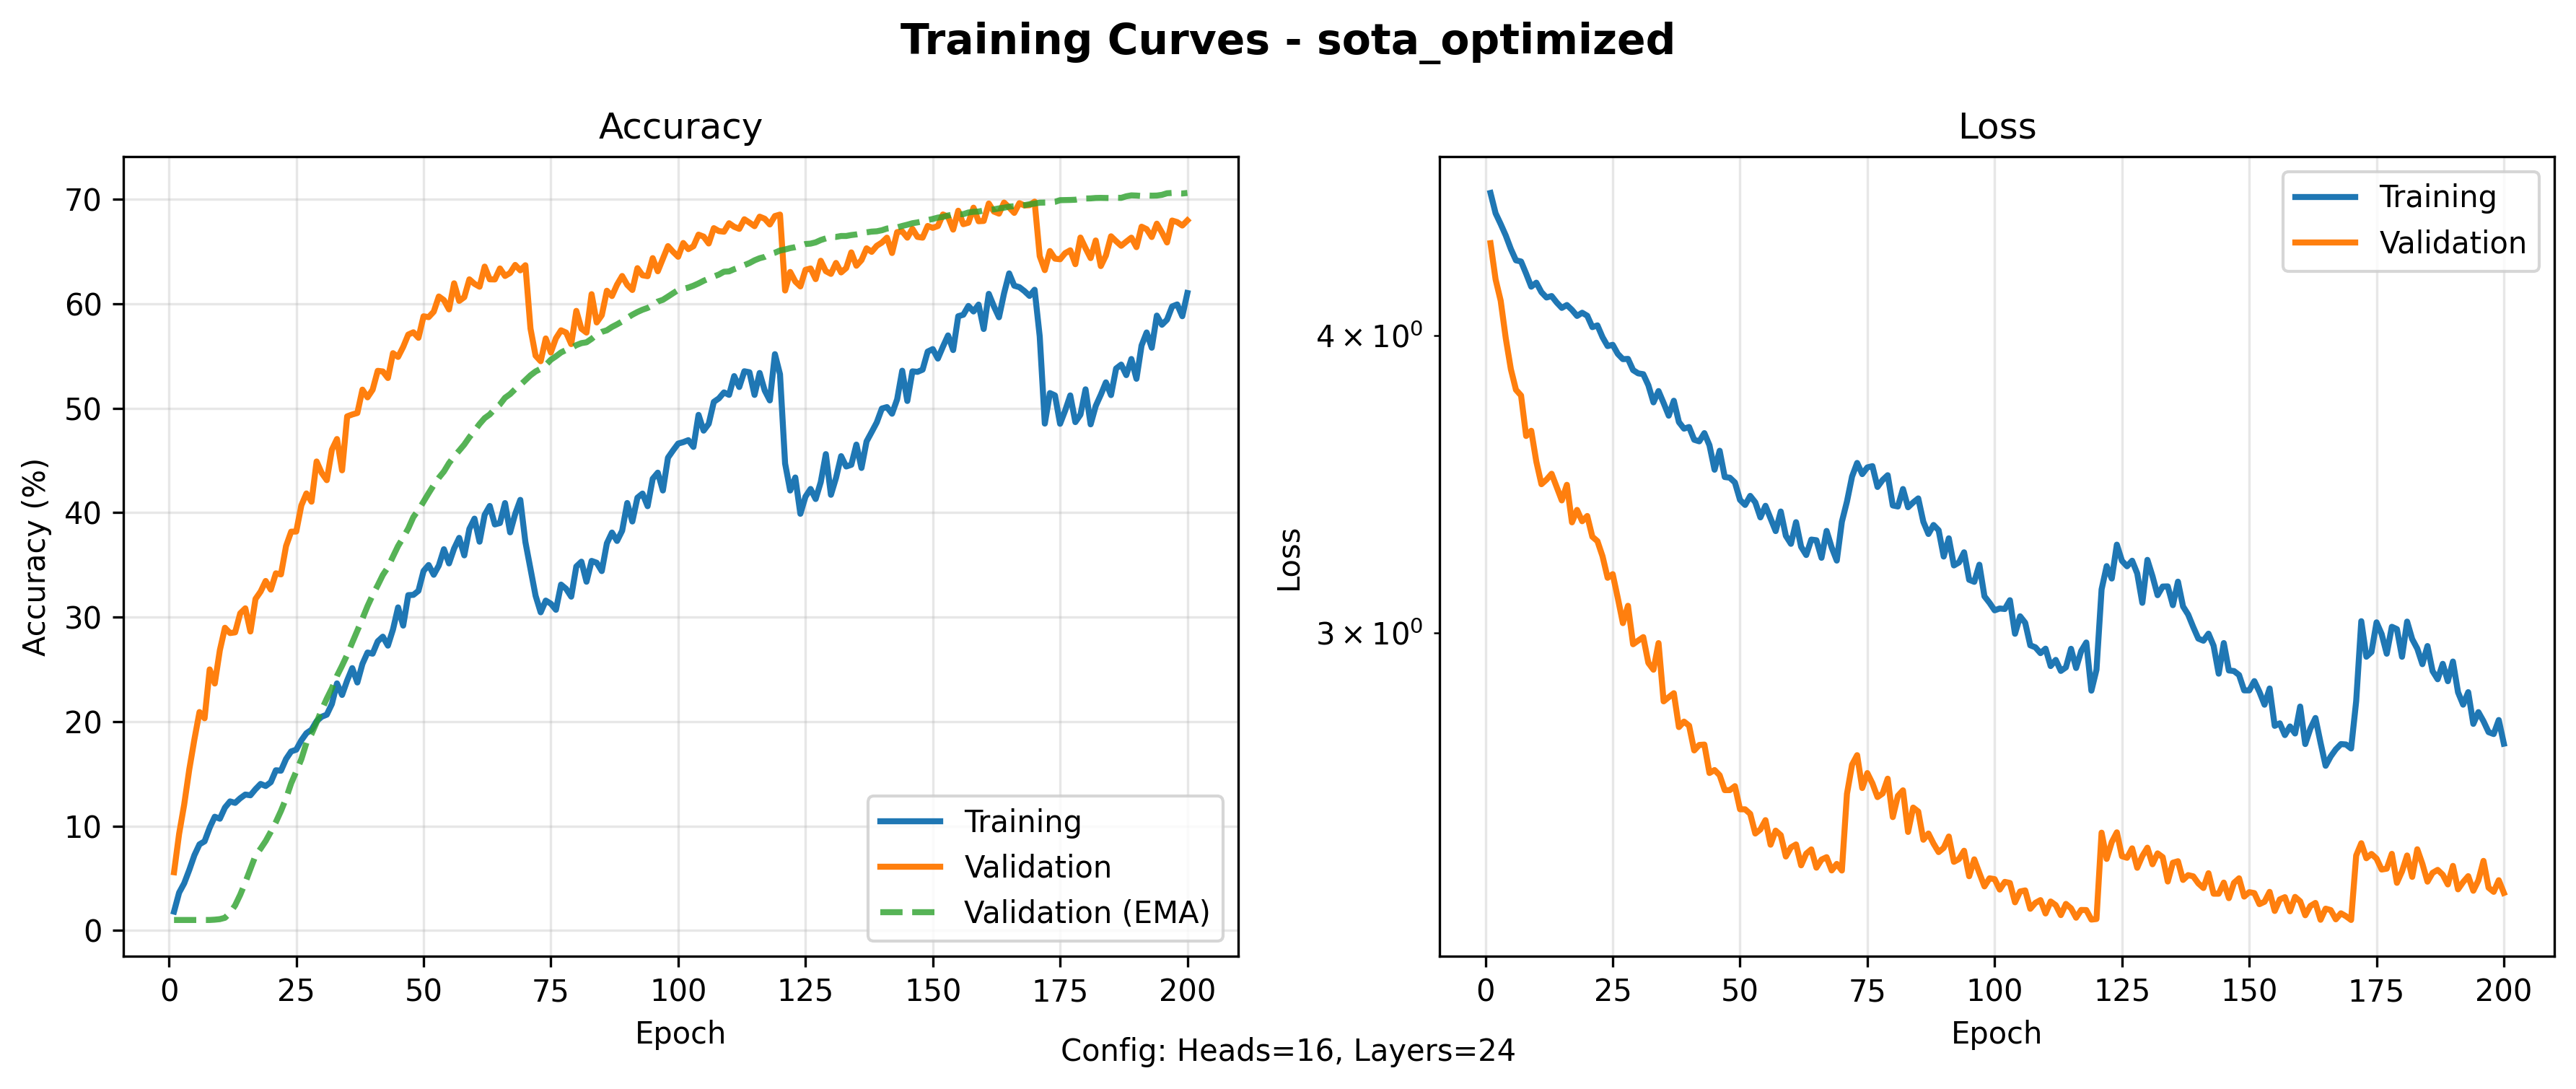
\includegraphics[width=0.8\textwidth]{curves_sota_optimized.png}
    \caption{Curvas detalhadas de treinamento do modelo SOTA otimizado. O padrão \textit{sawtooth} característico resulta do treinamento multi-escala (alternância entre resoluções 192/224/256 pixels), enquanto a curva EMA (linha tracejada) demonstra a suavização e estabilidade proporcionada pela técnica de Exponential Moving Average.}
    \label{fig:sota_curves}
\end{figure}

\bibliographystyle{IEEEtran}
\bibliography{references}

\end{document}
